
\documentclass[12pt,a4paper,final]{article}
\usepackage[utf8]{inputenc}
\usepackage[francais]{babel}
\usepackage[T1]{fontenc}
\usepackage{amsmath}
\usepackage{amsfonts}
\usepackage{amsthm}
\usepackage{color}
\usepackage{amssymb}
\usepackage{graphicx}
\usepackage{algorithm}
\usepackage{algorithmic}
\usepackage{fancyhdr}
\usepackage[fs]{umons-coverpage}
\usepackage{hyperref}

%%###### START CHANGE HERE ######
\author{S. Opsommer \& T. Watillon}
\title{Assemblage de fragments d’ADN Rapport de projet}
\umonsAuthor{\begin{tabular}{lll}
\textsc{Watillon} & Thibaut & THIBAUT.WATILLON@student.umons.ac.be\\
\textsc{Opsommer} & Sophie & SOPHIE.OPSOMMER@student.umons.ac.be\\
\end{tabular}}
%% The main title of your thesis
\umonsTitle{Assemblage de fragments d’ADN\\ - \\Rapport de projet}
%% The sub-title of your thesis
\umonsSubtitle{Projet réalisé dans le cadre \\de la 1er Master en Sciences informatique \\pour le cours d'\og Algorithmique et bioinformatique \fg}
%% Your supervisor(s)
\umonsSupervisor{\begin{tabular}{ll}
\textit{Titulaire} : & O. \textsc{Delgrange} \\
\textit{Assistant} : & D. \textsc{Maslowski} \\
\end{tabular}}
%% The date (or academic year)
\umonsDate {\hfill Ann\'ee Acad\'emique 2014-2015}
%%###### END CHANGEMENT ######

\newcommand{\smalltitle}[1]{\bigskip\large\textbf{#1}\par\normalsize\medskip}
\newcommand{\partitle}[1]{\bigskip\textit{\underline{#1}}\par\medskip}

\newtheorem{defi}{Définition}
\newtheorem{note}{Note}
\newtheorem{prop}{Propriété}
\newtheorem{exemple}{Exemple}
\newtheorem{corollaire}{Corollaire}
\newtheorem{lemme}{Lemme}
\newtheorem{rem}{Remarque}
\newtheorem{thm}{Théorème}

\fancyhf{}
\chead{\leftmark}
\rfoot{\thepage}

\begin{document}

\umonsCoverPage
\pagebreak

\pagestyle{fancy}

\newpage
\thispagestyle{empty}
\vspace*{\stretch{1}}
\begin{abstract}
\addcontentsline{toc}{section}{Résumé}
Ce \emph{rapport} est rendu dans le cadre du cursus de première année de \og Master en Sciences Informatiques\fg  pour le cours de \emph{Algorithmique et bioinformatique} (dont le titulaire est Mr. \emph{O. Delgrange} et l'assistant est Mr. \emph{D. Maslowski} en année académique 2014-2015) . Le but de ce rapport est de présenter les résultats de l'implémentation du projet.
\end{abstract}
\vspace*{\stretch{1}}

\thispagestyle{empty}
\newpage
\tableofcontents
\newpage

%%###### LE RAPPORT COMMENCE ICI ######
%\smalltitle{Note préliminaire}
%\addcontentsline{toc}{section}{Note préliminaire}
%La rédaction de ce document est basé sur le livre \textit{Introduction to algorithme}~\cite{intro_to_algo}

\section{Introduction}
\subsection{Problème posé}
Ce projet consiste à développer un programme informatique qui a la particularité de pouvoir, à partir d'une collection de fragments (de longueur variable), créer un contig le plus petit possible avec tous les fragments (ou leur complémentaire inversé).

\subsection{Les données}
\subsubsection{En entrée}
Les fragments sont fournis par le biais d'un fichier au format \og .FASTA \fg .\\
La structure d'un tel format est tel que : un fichier contient au moins 1 fragment. Chaque fragment est de la forme : 
\begin{table}[!ht]
\centering
\begin{tabular}{|l|}
	\hline
	> identifiant-de-la-séquence $[$commentaire$]$\\
	suite-de-caractères\\
	$[$suite-de-caractères$]$ \\
	$[$suite-de-caractères$]$ \\
	. . .\\
	\hline
\end{tabular}
\end{table}

Notons que il doit-être possible d'introduire des fichiers simplifié, c'est-à-dire des fichiers où le sens de lecture des fragments est connu. Pour ceux-ci, il ne faut donc par calculer les fragments complémentaire inversé.

\subsubsection{En sortie}
Les fichiers généré par le programme se trouve à la racine du programme. Ils sont au format : 

\begin{table}[!ht]
\centering
\begin{tabular}{|l|}
	\hline
	> nom nom-etudiant Collection num-collection Longueur longueur-sequence-cible \\
	suite-de-caractères\\
	\hline
\end{tabular}
\end{table}

\subsection{Etapes clés}
Les étapes clés du projet sont les suivantes : (chronologiquement)
\begin{enumerate}
\item Compréhension du projet à réaliser
\item Lecture du fichier de fragments
\item Construction du graphe
\item Implémentation de l'algorithme Greedy 
\item Construction de la super chaine 
\item Ecriture du résultat dans un fichier
\end{enumerate}

%%%%%%%%%%%%%%%%%%%%%%%%%%%%%%%%%%%%%%%%%%%%%%%%%%%%%%%%%%%%
\newpage
\section{Implémentation}
\subsection{Structures de données}

Lors de la lecture des fichiers, les fragments sont insérés dans des objets \textit{Fragment}.\medskip

Ces objets \textit{Fragment} sont ensuite insérés dans des objets \textit{Node} correspondant aux noeuds du graph de chevauchement.  Ces objets en plus de contenir un fragment contiennent aussi un booléen \textit{in} et un booléen \textit{out} nécessaire pour le \textit{Greedy}, une référence vers le noeud de son complémentaire inversé et une liste des noeuds dont les fragments sont inclus au fragment de ce noeud.\medskip

Pour appliquer l'algorithme \textit{Greedy} sur le graph, il faut tout d'abord que ce graph possède des arcs.  Pour ce faire, un objet \textit{Edge} a été créé et contient le noeud de début et le noeud de fin de cet arc ainsi qu'un objet \textit{Alignment} contenant les informations de l'alignement entre le fragment du noeud source et le fragment du noeud destination.\medskip

L'objet \textit{Alignment} comprend donc : Le type d'alignement (préfixe, suffixe, inclu), le coût de l'alignement, l'indice du début de l'alignement, l'alignement du fragment du noeud source et l'alignement du fragment du noeud destination.\medskip

La dernière structure de données concerne le graph de chevauchement.  Il contient une liste des noeuds ainsi qu'une liste des arcs.

Les objects \textit{Fragment}, \textit{Node}, \textit{Edge}, \textit{Alignement}, \textit{AlignementType} et \textit{Graph} sont représenté à la figure \ref{UMLobj}.

\begin{figure}[!ht]
\centering
	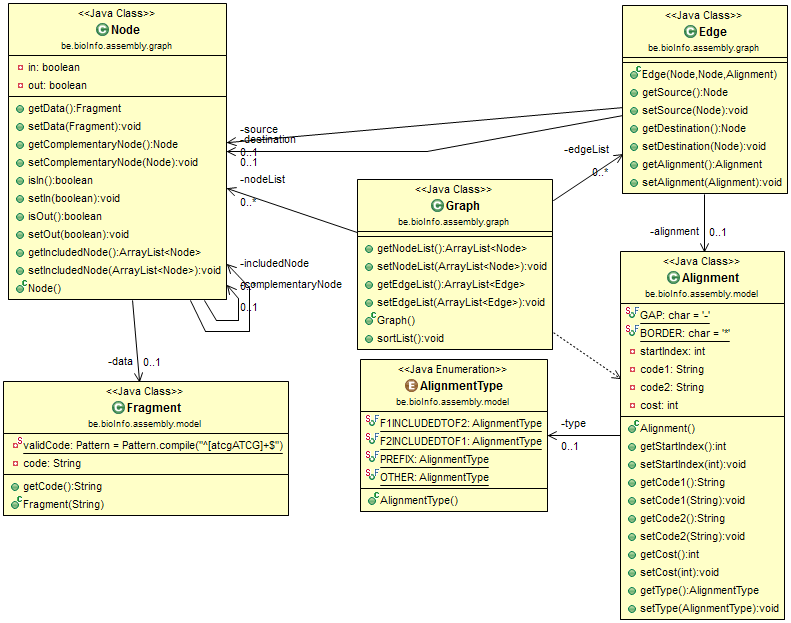
\includegraphics[width=0.8\textwidth]{images/classDiagram_Objects.png}
	\caption{\label{UMLobj}Visualisation des objects principaux}
\end{figure}

\subsection{Construction du graph de chevauchement}

Cette partie de l'application est la plus gourmande en terme de ressources et consiste à créer les arcs du graph de chevauchement.\medskip

En effet, lorsque nous avons $n$ fragments et que nous devons calculer les complémentaires inversés, $n*(n-2)$ arcs sont à créer.  Si les fragments complémentaires inversés ne sont pas à calculer, $n*(n-1)$ arcs sont à créer.\medskip

Pour réduire le temps de calcul, nous appliquons donc le multithreading.\medskip

Deux contraites sont à respecter lors de la construction des arcs.  La première est qu'il ne faut pas créer d'arc entre un noeud et son complémentaire inversé.  La seconde étant qu'il ne faut pas créer un arc ayant comme source et destination le même noeud.  D'où le $n*(n-2)$\medskip

La création des arcs introduit aussi l'algorithme de l'alignement semi-global.\medskip

\subsection{Algorithme de l'alignement semi-global}

Lors de la création des arcs, l'alignement entre les deux fragments concernés doit être calculé pour attribuer un coût à l'arc et pour déterminer le type d'alignement entre ces deux fragments.\medskip

Lors de la construction d'un arc de $n_1$ à $n_2$, la matrice calculée et utilisée pour déterminer l'alignement entre les deux fragments sera également utilisée pour déterminer l'alignement de l'arc allant de $n_2$ à $n_1$.\medskip

Pour construire l'alignement de $n_1$ à $n_2$, on se positionne sur la valeur maximale de la dernière ligne de la matrice tandis que pour construire l'alignement de $n_2$ à $n_1$, on se positionne sur la valeur maximale de la dernière colonne.\medskip

Une fois l'algorithme exécuté, nous obtenons deux chaînes de caractères représentant l'alignement entre les fragments : \medskip

ACTGCGTA****** : Fragment du noeud source (f1)\medskip

****CGTAAAA*** : Fragment du noeud destination (f2) \medskip


Grâce à ces deux chaînes de caractères, nous pouvons déterminer le type d'alignement qui sera nécessaire lors de l'exécution du \textit{Greedy}\medskip

%Si le premier et dernier caractère de la première chaîne est '*', alors f1 est inclu à f2.\medskip
%Sinon, si le premier caractère de f1 est '*' et son dernier n'est pas '*', alors f1 est préfixe de f2.\medskip
%Sinon, si le premier caractère de f1 n'est pas '*' et son dernier caractère l'est, alors f1 est suffixe de f2.\medskip
%Sinon,  si le premier caractère de f2 est '*' ou son dernier caractère est '*', alors f2 est inclu à f1.\medskip
%Sinon les deux fragments sont égaux.\medskip

Il est également possible de déterminer la position du début de l'alignement qui sera utile lors de la construction de la séquence.\medskip

Dans l'exemple, le début de l'alignement se trouve à la 4\up{ème} position dans la seconde chaîne.\medskip

Une fois les arcs construits et les caractéristiques des alignements connues, l'algorithme \textit{Greedy} peut être appliqué sur les arcs du graph.\medskip

\subsection{Algorithme Greedy}

Avant d'appliquer le \textit{Greedy}, les arcs doivent tout d'abord être triés par ordre décroissant en fonction de leur coût.\medskip

Pour ce faire, la méthode \textit{Collection.sort()} est utilisé sur la liste des arcs.\medskip

Le problème lors de ce tri est que les arcs ayant le même coût ont des positions à chaque fois différentes lors de l'exécution de\textit{Collection.sort()} ce qui fait que les arcs sélectionnés par \textit{Greedy} varient à chaque exécution de l'application.\medskip

L'algorithme a dû être modifié pour gérer les fragments inclus.\medskip

Pour ce faire, lors du traitement d'un arc $n_1$ --> $n_2$, si $n_1$ est inclu à $n_2$, le noeud $n_1$ est inséré dans la liste des fragments inclus à $n_2$.  De plus, il faut empécher de prendre par la suite le noeud $n_1$ et son complémentaire inversé en mettant ses booléen $in$ et $out$ à $TRUE$ et en insérant $n_1$ et son complémentaire inversé dans l'ensemble de $n_2$.  Cela est uniquement faisable si le noeud $n_1$ n'est pas déjà un noeud destination d'un arc choisit par \textit{Greedy} aussi non il serait impossible de reformer la séquence. \medskip

Mainenant, si $n_2$ est inclu à $n_1$, le noeud $n_2$ est inséré dans la liste des fragments inclus à $n_1$.  Il faut également empécher de prendre par la suite le noeud $n_2$ et son complémentaire inversé en mettant ses booléen $in$ et $out$ à $TRUE$ et en insérant $n_2$ et son complémentaire inversé dans l'ensemble de $n_1$.  Ici, cela est uniquement faisable si le noeud $n_2$ n'est pas déjà un noeud source d'un arc choisit par \textit{Greedy}.\medskip

Concernant les arcs dont les fragments ne sont pas inclus, il faut empêcher le noeud source d'être le noeud source d'un autre arc et d'empêcher le noeud destination d'être le noeud destination d'un autre arc.  Il faut également empêcher de prendre des arcs ayant comme noeuds les complémentaires inversés des noeuds déjà choisi par \textit{Greedy}.  Cela se fait via les booléens \textit{in} et \textit{out}.  Il ne faut également pas oublier de mettre tous ces noeuds dans le même ensemble (complémentaires inversés compris).\medskip

Une fois l'algorithme du \textit{Greedy} terminé, la liste des meilleurs arcs est disponible pour construire la séquence.

\subsection{Construction de la séquence}

Le but est, pour une séquence de taille N, de créer N tableaux où le tableau numéro $i$ contient le nombre de fois que les nucléotïdes A, C, T, G et les gaps sont présents à la $i^{eme}$ position dans la séquence. A noter que les tableaux contiendrons une cellule permettant de savoir si à la position $i$, nous sommes en présence ou non d'un gap.  Cela permettra de propager les gaps vers le bas.\medskip

\begin{figure}[!ht]
\centering
	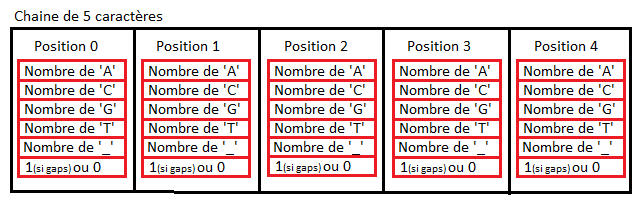
\includegraphics[width=1\textwidth]{images/table.png}
	\caption{\label{table}Visualisation des tableaux}
\end{figure}

Une fois tous les arcs traités, pour reconstruire la séquence, il suffira de regarder dans chaque tableau quel est le symbole le plus représenté et ce symbole sera celui à insérer dans la séquence à la position $i$.  A noter que pour empécher d'avoir le même nombre d'occurences de plusieurs symboles à la position $i$ et ainsi effectuer un choix aléatoire, on utilise le score de l'alignement (coût de l'arc) comme valeur à insérer dans le tableau.\medskip

La première étape consiste à trouver l'arc débutant la séquence c'est-à-dire, l'arc dont le noeud source n'est la destination d'aucun arc et donc le noeud de destination est aussi la source d'un autre arc.%est lié qu'au noeud destination et dont le noeud destination n'est lié qu'au noeud source de cet arc et à un noeud source d'un autre arc.  
Autrement dit, les booléen $in$ et $out$ du noeud source de cet arc doivent valoir respectivement $FALSE$ et $TRUE$  et ceux du noeud destination doivent valoir $TRUE$ et $TRUE$.\medskip

Une fois cet arc trouvé, on le traite et une fois cet arc traité, on cherche l'arc dont le noeud source équivaut au noeud destination de l'arc venant d'être traité pour ainsi former une chaîne.\medskip

Lors de la construction de la séquence, deux éléments importants doivent être pris en compte : la propagation des gaps vers les fragments précédents et la propagation des gaps vers les fragments futurs.\medskip

En effet, lors de la gestion d'un arc $n_1$-->$n_2$, si la chaîne de caractères du fragment de $n_1$ possède un gap à la $i^{eme}$ position cela signifie que le caractère $i+1$ de cette chaîne correspond au caractère à la position $i$ dans la séquence.  Il s'agit donc de décaler vers la droite le tableau correspondant au $i^{eme}$ caractère de la séquence ainsi que tous les tableaux correspondant aux caractères se trouvant après le $i^{eme}$ caractère et d'insérer un nouveau tableau à la position $i$.  Un exemple de ce type de propagation de gaps est visible à la figure \ref{gapPrecedent}.\medskip

Un problème équivalent survient lorsque dans l'arc $n_1$-->$n_2$, la chaîne de caractère du fragment de $n_2$ possède un gap à la $i^{eme}$ position.  Les futurs fragments à insérer dans la séquence devront faire correspondre leur $i^{eme}$ caractère au $i+1^{eme}$ caractère de la séquence.  Un exemple de ce type de propagation de gaps est visible à la figure \ref{gapSuivant}.\medskip

\begin{figure}[!ht]
\centering
	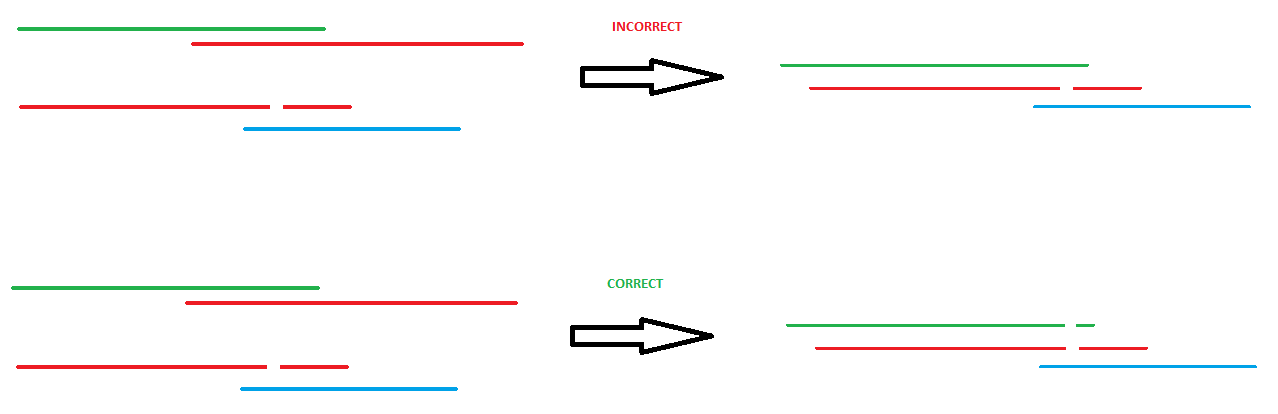
\includegraphics[width=1\textwidth]{images/gapPrecedent.png}
	\caption{\label{gapPrecedent}Exemple de propagation d'un gap vers les fragments précédents}
\end{figure}

\begin{figure}[!ht]
\centering
	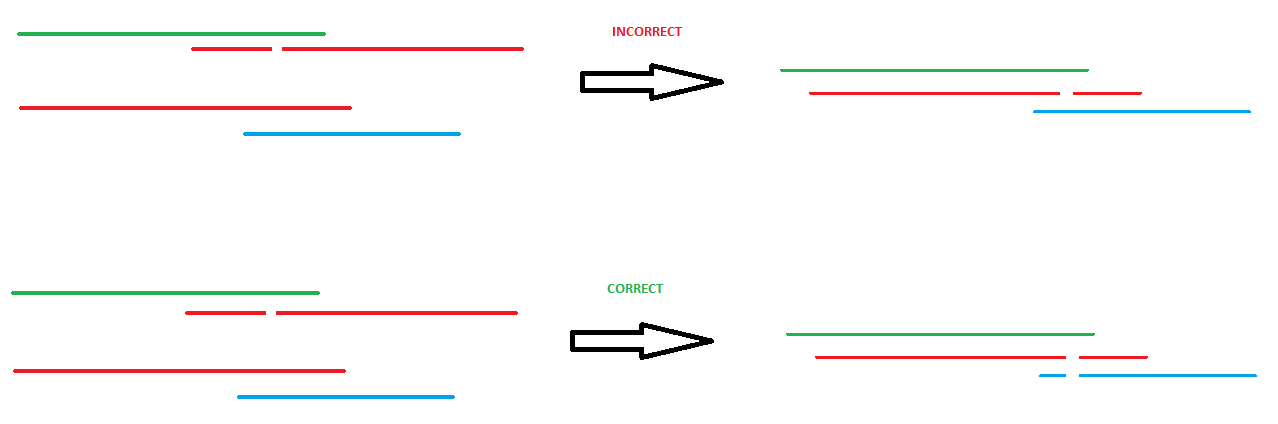
\includegraphics[width=1\textwidth]{images/gapSuivant.png}
	\caption{\label{gapSuivant}Exemple de propagation d'un gap vers les fragments futurs}
\end{figure}

%%%%%%%%%%%%%%%%%%%%%%%%%%%%%%%%%%%%%%%%%%%%%%%%%%%%%%%%%%%%
\newpage
\section{Résultats}
Voici les résultats obtenus : 

\subsection{Collection 1}
Les deux résultats présentés à la figure \ref{coll1} sont les deux meilleurs résultats que nous ayons obtenu au court de nos nombreux test. On y voit que l'ensemble (ou presque) de la séquence cible a été retrouvée, cependant (tel que énoncé dans les points faibles), on observe aussi que de nombreux fragment n'ont pas été compris dans la partie 'cible' de la séquence (et ont été placé avant et après).

\begin{figure}[!ht]
	\centering
	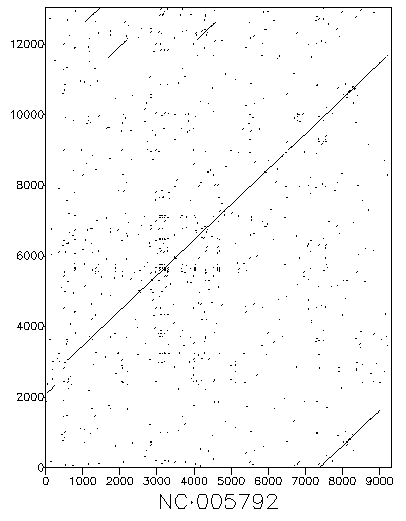
\includegraphics[width=0.4\textwidth]{images/collection1/collection1_2.png}
	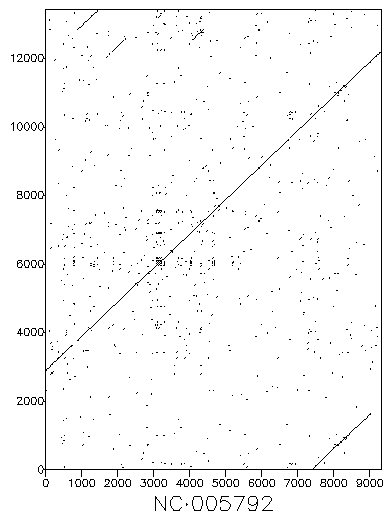
\includegraphics[width=0.4\textwidth]{images/collection1/collection1_16.png}
	\caption{\label{coll2}Résultats de la comparaison entre les fichiers générés et le fichier cible de la collection 1}
\end{figure}

\subsection{Collection 4}
Les deux résultats présentés à la figure \ref{coll4} sont les deux meilleurs résultats que nous ayons obtenu au court de nos nombreux test. On y observe que les résultats sont un peu moins bons que pour la collection 1. En effet ici, la partie cible est segmentée en plus de morceaux et ces morceux sont plus éparpillé au sein du contig. Mais, notons tout de même que l'ensemble (ou presque) de la séquence cible a été retrouvée( bien que de nombreux fragment n'ont pas été compris dans la partie 'cible' de la séquence).

\begin{figure}[!ht]
	\centering
	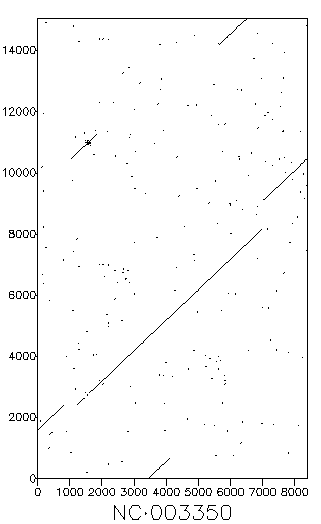
\includegraphics[width=0.4\textwidth]{images/collection4/collection4_2.png}
	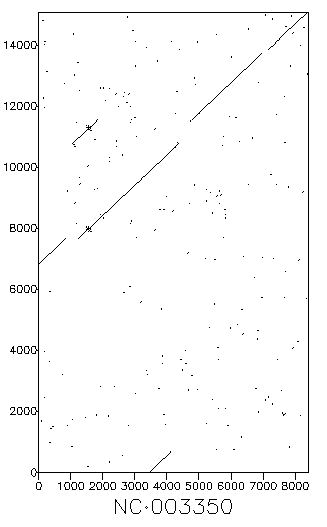
\includegraphics[width=0.4\textwidth]{images/collection4/collection4_3.png}
	\caption{\label{coll4}Résultats de la comparaison entre les fichiers générés et le fichier cible de la collection 4}
\end{figure}

\subsection{Collection 5}
Les trois résultats présentés à la figure \ref{coll5} sont nos meilleurs résultats pour cette collection. On y observe que les résultats sont encore un peu moins bons que pour la collection 4. En effet en plus d'une segmentation de la partie cible qui augmente, l'ensemble de la séquence cible n'est plus retrouvée.

\begin{figure}[!ht]
	\centering
	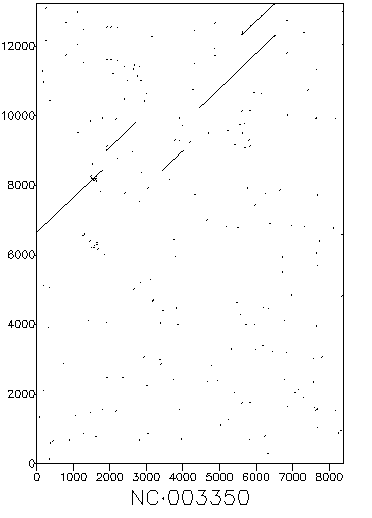
\includegraphics[width=0.3\textwidth]{images/collection5/collection5_1.png}
	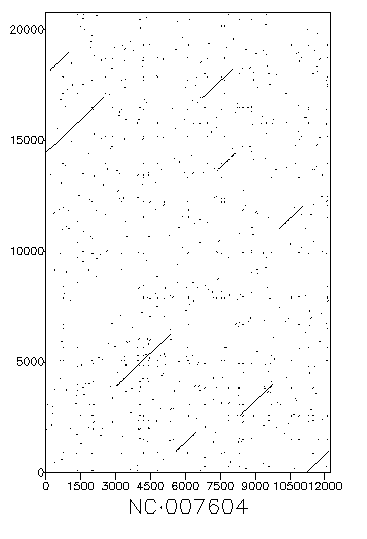
\includegraphics[width=0.3\textwidth]{images/collection5/collection5_3.png}
	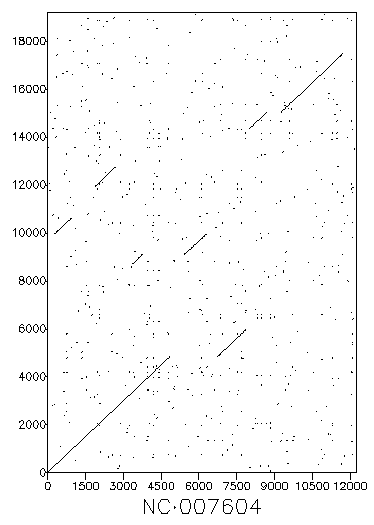
\includegraphics[width=0.3\textwidth]{images/collection5/collection5_9.png}
	\caption{\label{coll5}Résultats de la comparaison entre les fichiers générés et le fichier cible de la collection 5}
\end{figure}


\subsection{Collection S1}
La collection S1 correspond aux mêmes fragments que la collection 1 seulement les fragments complémentaires et inversés ne doivent pas êtres calculés, ils sont fournis.

La figure \ref{collS1} est notre meilleur résultat. Il est, de façon évidente, bien meilleur que toutes les autres comparaisons préalables. On y voit que l'ensemble (ou presque) de la séquence cible a été retrouvée, et en plus, la longeur de notre résultat est comparable à la longueur de la séquence cible.

\begin{figure}[!ht]
	\centering
	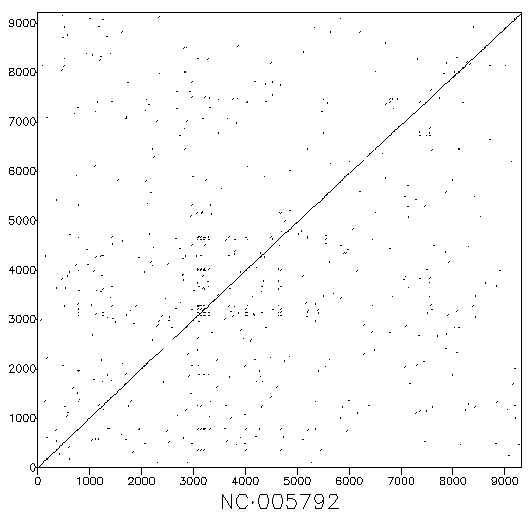
\includegraphics[width=0.5\textwidth]{images/collectionS1/collectionS1.png}
	\caption{\label{collS1}Résultat de la comparaison entre le fichier généré et le fichier cible de la collection S1}
\end{figure}

\subsection{Collection S2}
La figure \ref{collS2} est notre meilleur résultat. Il est, de façon évidente, bien meilleur que toutes les autres comparaisons préalables réalisée sur les fichiers non simplifié et comparable au résultat du fichier de la collection S1. On y voit que l'ensemble (ou presque) de la séquence cible a été retrouvée, et en plus, la longeur de notre résultat est comparable à la longueur de la séquence cible.

\begin{figure}[!ht]
	\centering
	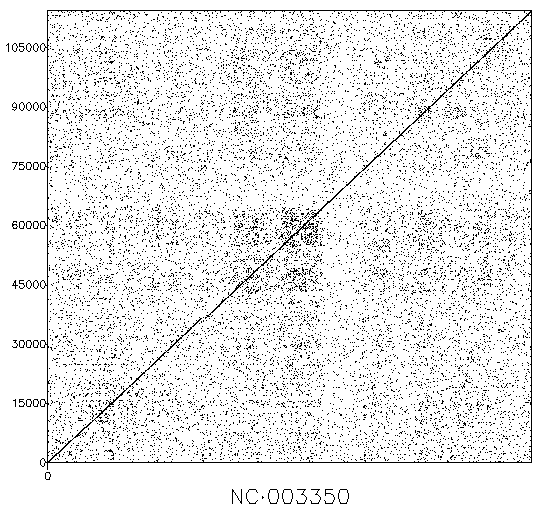
\includegraphics[width=0.5\textwidth]{images/collectionS2/collectionS2.png}
	\caption{\label{collS2}Résultat de la comparaison entre le fichier généré et le fichier cible de la collection S2}
\end{figure}

%%%%%%%%%%%%%%%%%%%%%%%%%%%%%%%%%%%%%%%%%%%%%%%%%%%%%%%%%%%%
\newpage
\section{Problèmes rencontrés}

Nous avons rencontrés de nombreux problèmes et ce à chaque étape de la réalisation de l'application.\medskip

La première étant lors de l'implémentation de l'algorithme de l'alignement semi-global et la détermination du type de l'alignement.  Nous avons longuement essayer de déterminer le type de l'alignement (préfixe, suffixe, inclusion) via la matrice de l'alignement mais cette méthode donnait des mauvais résultats lorsque l'alignement contenait des gaps.  Nous nous sommes alors basé sur les chaînes de caractères représentant l'alignement et nous avons obtenus de meilleurs résultats.\medskip

La seconde difficulté était au niveau de l'algorithme \textit{Greedy} et la gestion des fragments inclus.  Il nous a fallu un certains temps avant d'arriver à les gérer correctement.\medskip

La dernière difficulté concerne la construction de la séquence en elle même.  Cette étape fut la plus dure car de nombreux éléments étaient à prendre en compte.  Comment gérer les gaps, les fragments inclus, comment reconstituer une chaine via les arcs,...

%%%%%%%%%%%%%%%%%%%%%%%%%%%%%%%%%%%%%%%%%%%%%%%%%%%%%%%%%%%%
\newpage
\section{Logiciel}

\subsection{Points forts}

Un point fort du logiciel est qu'il est multithreadé au niveau de la construction des arcs du graph permettant ainsi de gagner un temps considérable.

Un seconde point fort est qu'il propose une interface graphique permettant d'aller directement sélectionner le fichier à traiter sans devoir insérer son chemin d'accès.

\subsection{Points faibles}

Un point faible du logiciel est la variabilité des résultats à chaque exécution de l'application.  Cela vient du fait que lors du tri des arcs par ordre décroissant en fonction de leur coût, la méthode \textit{Collection.sort()} trie différement les arcs ayant le même coût.\medskip


Un second point faible est que les fragments inclus n'ont pas été traités lors de la construction de la séquence par manque de temps bien qu'ils ont été détecté par \textit{Greedy}.

\subsection{Erreurs connues}

Une erreur connue concerne la longueur de la séquence obtenue.  Nous ne savons pas pourquoi la séquence contient beaucoup plus de caractère que la séquence cible.

%%%%%%%%%%%%%%%%%%%%%%%%%%%%%%%%%%%%%%%%%%%%%%%%%%%%%%%%%%%%
\newpage
\section{Répartition des tâches}

\begin{table}[!ht]
\centering
\begin{tabular}{|l|l|l|}
	\hline
	Tâche & Réalisé par Thibaut & Réalisé par sophie\\
	\hline
	Compréhension du projet à réaliser & 50\% & 50\% \\
	Lecture du fichier de fragments & 90\% & 10\% \\
	Construction du graphe & 90\% & 10\% \\
	Implémentation de l'algorithme Greedy  & 90\% & 10\% \\
	Construction de la super chaine  & 90\% & 10\% \\
	Ecriture du résultat dans un fichier & 75\% & 25\% \\
	Rédaction du rapport  & 50\% & 50\% \\ % 7 pages par thibaut
\end{tabular}
\end{table}

%%%%%%%%%%%%%%%%%%%%%%%%%%%%%%%%%%%%%%%%%%%%%%%%%%%%%%%%%%%%
\newpage
\section{Conclusion} 

\bibliographystyle{plain}
\bibliography{reference}

\end{document} 